% select theme
\documentclass[t,8pt,aspectratio=169]{beamer}

% ====================================================
% ====================================================
% USEPACKAGES
% ====================================================
% ====================================================

\usepackage[T1]{fontenc}
\usepackage[utf8]{inputenc}
\usepackage[english]{babel}

% tables
\usepackage{tabularx}
\usepackage{colortbl}
\usepackage{multirow}
\usepackage{makecell}

% tikz and colors
\usepackage{tikz}
\usepackage{xcolor}
\usepackage{pgf-pie}
\usepackage{pgfplots}
\usepackage{pgfplotstable}
\usepackage{tikzsymbols}

\usetikzlibrary{calc}
\usetikzlibrary{trees}
\usetikzlibrary{patterns}
\usetikzlibrary{shadings}
\usetikzlibrary{positioning}
\usetikzlibrary{intersections}
\usetikzlibrary{decorations.pathreplacing}

\usetikzlibrary{arrows}
\usetikzlibrary{arrows.meta}

\usetikzlibrary{shapes}
\usetikzlibrary{shapes.arrows}
\usetikzlibrary{shapes.callouts}
\usetikzlibrary{shapes.symbols}
\usetikzlibrary{shapes.geometric}

\usepgfplotslibrary{patchplots}
\usepgfplotslibrary{fillbetween}

% boxes
\usepackage[many]{tcolorbox}

% math packages and fonts
\usepackage{bm}
\usepackage{ccfonts}
\usepackage{eulervm}
\usepackage{amsmath}
\usepackage{amsfonts}
\usepackage{amssymb}
\usepackage{amsthm}
\usepackage{mathtools}
\usepackage{nicefrac}
\usepackage{slashed}
\usepackage{bbold}
\usepackage{array}
\usepackage{cancel}

% algorithms and listings
\usepackage[ruled,vlined,linesnumbered]{algorithm2e}
\usepackage{listings}
\usepackage{setspace}

\tcbuselibrary{listings}
\tcbuselibrary{breakable}
\tcbuselibrary{skins}

% misc
\usepackage{soul}
\usepackage{pifont}
\usepackage{skull}
\usepackage{multicol}
\usepackage{animate}
\usepackage{cleveref}
\usepackage{hyperref}
\usepackage{wasysym}
\usepackage[absolute,overlay]{textpos}
\usepackage[hang,flushmargin]{footmisc}
\usepackage[framemethod=tikz]{mdframed} 				% provides frame for framed figure and framed table in theme_2

% ====================================================
% ====================================================
% COLOR DEFINITIONS
% ====================================================
% ====================================================

\definecolor{myblue1}{RGB}{35,119,189}
\definecolor{myblue2}{RGB}{95,179,238}
\definecolor{myblue3}{RGB}{129,168,207}
\definecolor{myblue4}{RGB}{26,89,142}

\definecolor{myred1}{RGB}{247,12,12}

% ====================================================
% ====================================================
% COMMON COMMANDS AND DEFINITIONS
% ====================================================
% ====================================================

% math definitions
% ====================================================
% argmin, argmax
\DeclareMathOperator*{\argmax}{arg\,max}
\DeclareMathOperator*{\argmin}{arg\,min}

% integration d
\newcommand*\diff{\mathop{}\!\mathrm{d}}

% independent sign
\newcommand{\indep}{\rotatebox[origin=c]{90}{$\models$}}

% vertical and horizontal bar
\newcommand*{\vertbar}{\rule[-1ex]{0.5pt}{2.5ex}}
\newcommand*{\horzbar}{\rule[.5ex]{2.5ex}{0.5pt}}

% math cancel sign
\newcommand\hcancel[2][black]{\setbox0=\hbox{$#2$}%
	\rlap{\raisebox{.45\ht0}{\textcolor{#1}{\rule{\wd0}{1pt}}}}#2}

% column type for matrices
\newcolumntype{C}[1]{>{\centering\arraybackslash}p{#1}}

% table definitions
% ====================================================
% centered X column in tabularx
\newcolumntype{Y}{>{\centering\arraybackslash}X}

% font commands
% ====================================================
% style of hyperlinks
\newcommand{\linkstyle}[1]{\underline{\smash{\texttt{#1}}}}

% slide architecture
% ====================================================
% divide frame into two parts
\newcommand{\divideTwo}[4]{
	\begin{minipage}{#1\textwidth}
		#2
	\end{minipage}
	\hfill
	\begin{minipage}{#3\textwidth}
		#4
	\end{minipage}
}

% divide frame into two parts (start on top)
\newcommand{\divideTwoTop}[4]{
	\begin{minipage}[t]{#1\textwidth}
		#2
	\end{minipage}
	\hfill
	\begin{minipage}[t]{#3\textwidth}
		#4
	\end{minipage}
}


% ====================================================
% ====================================================
% LAYOUT AND THEME
% ====================================================
% ====================================================

% adjust margin left and right
\setbeamersize{text margin left=25pt,text margin right=25pt}

% define colors
% ====================================================
\setbeamercolor{frametitle}{fg=black}
\setbeamercolor{itemize item}{fg=black}
\setbeamercolor{itemize subitem}{fg=black}
\setbeamercolor{caption name}{fg=black!80!white}
\setbeamercolor{section in toc}{fg=black}
\setbeamercolor{subsection in toc}{fg=gray!20!black}

% define fonts and sizes
% ====================================================
\setbeamerfont{frametitle}{series=\bf,size=\footnotesize}
\setbeamerfont{caption name}{series=\bf}
\setbeamertemplate{itemize/enumerate subbody begin}{\normalsize}
\setbeamertemplate{itemize/enumerate subsubbody begin}{\small}
\usefonttheme[onlymath]{serif}

% table of contents
% ====================================================
\makeatletter
\def\beamer@endinputifotherversion#1{}
\def\beamer@sectionintoc#1#2#3#4#5{{\large \vspace*{3mm} \textbf{#2} \hfill \textbf{#3} \par}}
\def\beamer@subsectionintoc#1#2#3#4#5#6{{\normalsize \hspace*{3mm} \textbf{#3} \hfill \textbf{#4} \par}}
\def\beamer@subsubsectionintoc#1#2#3#4#5#6#7{{\normalsize \hspace*{6mm} \textbf{#4} \hfill #5 \par}}
\makeatother

% define bullet points
% ====================================================
\setbeamertemplate{itemize item}[circle]
\setbeamertemplate{itemize subitem}{--}
\setbeamertemplate{itemize subsubitem}{\textcolor{black}{$\triangleright$}}
\setlength{\leftmargini}{3.5mm}
\setlength{\leftmarginii}{3.5mm}
\setlength{\leftmarginiii}{3.5mm}

% frametitle
% ====================================================
\setbeamertemplate{frametitle}{%
	\vspace*{1mm}
	\ifthenelse{\boolean{deeptoc}}{
		\ifnum\insertframenumber=\insertsectionstartpage%
			\vspace*{0.1mm}
    			\begin{tcolorbox}[
				skin=enhanced,
      				boxrule=0.6mm, boxsep=0mm,
     	   			lowerbox=ignored,
        			colback=orange!60!red, colframe=black,
        			borderline={0.5pt}{3pt}{black}, borderline={1pt}{2pt}{red}
    			]
        			\centering
        			\Huge\textbf\insertsectionhead\par
    			\end{tcolorbox}
		\fi%
	}{}
	\ifnum\insertframenumber=\insertsubsectionstartpage%
    		\vspace*{0.1mm}
    		\begin{tcolorbox}[
     		   	boxrule=0.4mm, boxsep=-0.5mm,
     	   		lowerbox=ignored,
     	   		colback=yellow!60!orange, colframe=black
    		]
        		\centering
        		\huge\textbf\insertsubsectionhead\par
   	 	\end{tcolorbox}
	\fi%
	\begin{tcolorbox}[
    		boxrule=0.2mm,
    		boxsep=0mm,
    		lowerbox=ignored,
    		colback=yellow, colframe=black
	]
    		\centering
    		\large\insertframetitle
	\end{tcolorbox}
	\vspace*{-2mm}
}

% header and Footer
% ====================================================

% header
\setbeamertemplate{headline}{
	% skip header line on first frame of section
	\ifnum\insertsectionstartframe=\insertframenumber%
     		\vskip-\headheight%
	\else
		\begin{beamercolorbox}[wd=\textwidth,ht=4mm,dp=1mm]{}
			\hspace*{25pt} \Fheadline \hspace{25pt}
		\end{beamercolorbox}
		\centerline{\rule{\linewidth}{.2pt}}
	\fi
}

\setbeamertemplate{footline}{%
	\centerline{\rule{\linewidth}{.2pt}}
	\begin{beamercolorbox}[wd=\textwidth,ht=2mm,dp=3mm]{}
		\hspace*{25pt} \Ffootline \hspace{25pt}
	\end{beamercolorbox}
}

% definition of header
\newcommand{\Fheadline}{
	\ifx\insertshorttitle\undefined
		\inserttitle
	\else
		\insertshorttitle
	\fi
	\hfill
	\insertsection
}

% definition of footer
\newcommand{\Ffootline}{
	\textbf{\insertauthor,~\insertinstitute,~\insertdate}
	\hfill
	\insertframenumber
}

% customize captions
% ====================================================
\setbeamertemplate{caption}{%
	\begin{tcolorbox}[
		colback=lightgray, colframe=black,
		width=.17\linewidth,
		height=17pt,
		boxrule=0.5pt, boxsep=-1pt
	]
		\textbf{\strut\insertcaptionname~\insertcaptionnumber%
		\usebeamertemplate{caption label separator}}%
	\end{tcolorbox}%
	\space%
	\begin{tcolorbox}[
		colback=lightgray, colframe=black,
		width=.82\linewidth,
		height=17pt,
		boxrule=0.5pt, boxsep=-1pt
	]
		\strut\insertcaption%
	\end{tcolorbox}%
}

% remove navigation symbols
\setbeamertemplate{navigation symbols}{}

% remove header line on first frame of section
% ====================================================
\makeatletter
\newcount\beamer@sectionstartframe
\beamer@sectionstartframe=1
\apptocmd{\beamer@section}{\addtocontents{nav}{\protect\headcommand{%
            \protect\beamer@sectionframes{\the\beamer@sectionstartframe}{\the\c@framenumber}}}
}{}{}
\apptocmd{\beamer@section}%
{\beamer@sectionstartframe=\c@framenumber\advance\beamer@sectionstartframe by1\relax}{}{}
\AtEndDocument{
	\immediate\write\@auxout{\string\@writefile{nav}%
        	{\noexpand\headcommand{\noexpand\beamer@sectionframes{\the\beamer@sectionstartframe}%
	{\the\c@framenumber}}}}
}{}{}

\def\beamer@startframeofsection{1}
\def\beamer@endframeofsection{1}
\def\beamer@sectionframes#1#2{%
    		\ifnum\c@framenumber<#1%
    		\else%
    			\ifnum\c@framenumber>#2%
    			\else%
    				\gdef\beamer@startframeofsection{#1}%
    				\gdef\beamer@endframeofsection{#2}%
    			\fi%
    		\fi%
}

\newcommand\insertsectionstartframe{\beamer@startframeofsection}
\newcommand\insertsectionendframe{\beamer@endframeofsection}
\makeatother

% ====================================================
% ====================================================
% COMMANDS AND GENERAL DEFINITIONS
% ====================================================
% ====================================================

% variable definitions
% ====================================================
% variable deeptoc (deep or flat table of contents)
\newcommand{\dwDeepToc}[1]{
	\newboolean{deeptoc}
	\setboolean{deeptoc}{#1}
}

% adjust font
% ====================================================
\renewcommand*{\familydefault}{\sfdefault}

% framed floatings
% ====================================================
\newmdenv[
	innerlinewidth=0.05pt,
	roundcorner=4pt,
	linecolor=black,
	innerleftmargin=6pt,
	innerrightmargin=6pt,
	innertopmargin=6pt,
	innerbottommargin=6pt
]{mybox}

\newmdenv[
	innerlinewidth=0.05pt,
	roundcorner=4pt,
	linecolor=black,
	innerleftmargin=0pt,
	innerrightmargin=0pt,
	innertopmargin=0pt,
	innerbottommargin=-1pt
]{mytablebox}

% framed figure
\newcommand{\dwFigure}[3]{
	\begin{figure}
		\begin{mybox}
			\centering #1
  		\end{mybox}
  		\vspace{-4mm}
  		\caption{#2}
  		\label{#3}
	\end{figure}
	\vspace{-3mm}
}

% framed table
\newcommand{\dwTable}[4]{
	\begin{table}
		\begin{mytablebox}
			\renewcommand{\arraystretch}{#4} #1
		\end{mytablebox}
		\vspace{-2.5mm}
		\caption{#2}
		\label{#3}
	\end{table}
}

% sections and subsections
% ====================================================
% section command
\newcommand{\dwSection}[1]{
	\ifthenelse{\boolean{deeptoc}}{
		\section{#1}
	}{
		\section{#1}
		\subsection*{#1}
	}
}

% subsection command
\newcommand{\dwSubsection}[1]{\subsection{#1}}

% header
% ====================================================
% green header
\newcommand{\dwHeader}[1]{%
	\begin{tcolorbox}[
		boxrule=0.2mm, boxsep=-1mm,
		lowerbox=ignored,
		colback=green, colframe=black,
		hbox
	]
		\textbf{#1}
	\end{tcolorbox}
}

% alert box / info box
% ====================================================
\newcommand{\dwAlertBox}[1]{
	\vspace*{2mm}\hspace*{0.25mm}
	\begin{minipage}[c]{0.05\textwidth}
		\begin{tikzpicture}[rotate=180, transform shape]\thicki\end{tikzpicture}
	\end{minipage}
	\hfill
	\begin{minipage}[c]{0.92\textwidth}
		\begin{mybox}
			\textcolor{red}{\textbf{#1}}
		\end{mybox}
	\end{minipage}
}

\newcommand{\dwInfoBox}[1]{
	\vspace*{2mm}\hspace*{0.25mm}
	\begin{minipage}[c]{0.05\textwidth}
		\begin{tikzpicture}\thicki\end{tikzpicture}
	\end{minipage}
	\hfill
	\begin{minipage}[c]{0.92\textwidth}
		\begin{mybox}
			\textcolor{blue}{\textbf{#1}}
		\end{mybox}
	\end{minipage}
}

\newcommand{\thicki}{
	\draw[thick,fill=lightgray] (4.2,0) -- (4.5,0.5) -- (4.8,0) -- (4.2,0) -- cycle;
	\fill (4.45,0.05) rectangle (4.55,0.25);
	\fill (4.50,0.34) circle (1.5pt);
}

% custom itemize environment
% ====================================================
\let\tempone\itemize
\let\temptwo\enditemize
\renewenvironment{itemize}{\vspace*{1.5mm}\tempone\addtolength{\itemsep}{0.5\baselineskip}}{\temptwo}
\let\tempthree\enumerate
\let\tempfour\endenumerate
\renewenvironment{enumerate}{\vspace*{1.5mm}\tempthree\addtolength{\itemsep}{0.5\baselineskip}}{\tempfour}

% frames
% ====================================================
\newenvironment{dwHeaderFrame}[1]{
	\subsubsection{#1}
	\begin{frame}{#1}
}{
	\end{frame}
}

% special pages
% ====================================================
% title page
\newcommand{\dwPrintTitle}{
	{\usebackgroundtemplate{%
		\tikz[overlay,remember picture] \node[opacity=0.9, at=(current page.center)] {
  			
\includegraphics[height=\paperheight,width=\paperwidth]{../03_img/processor_red.jpg}
		};
	}
	\begin{frame}[plain]
		\begin{center}
			\begin{tcolorbox}[
				skin=enhanced,
	      			boxrule=0.6mm, boxsep=0mm,
				lowerbox=ignored,
				colback=orange!60!red, colframe=black,
				borderline={0.5pt}{3pt}{black}, borderline={1pt}{2pt}{red},
				width=\textwidth
			]
				\centering
				\Huge\textbf{\inserttitle}
			\end{tcolorbox}
			\vspace*{1.4cm}
			\begin{tcolorbox}[width=0.5\textwidth]
				\centering
				\textbf{\insertauthor} \\[2mm]
				\insertinstitute \\[2mm]
				\insertdate
			\end{tcolorbox}
			
			\begin{textblock}{1}(1,13.5)
				
\includegraphics[scale=0.04]{../03_img/logo_dhbw}
			\end{textblock}
		\end{center}
	\end{frame}}
}

% table of contents
\newcommand{\dwPrintToc}[1]{
	{\makeatletter
   		\setbeamertemplate{headline}[default]
   		\def\beamer@entrycode{\vspace*{-\headheight}}
	\makeatother

	\begin{frame}[allowframebreaks]
		\begin{tcolorbox}[
			skin=enhanced,
      			boxrule=0.6mm, boxsep=0mm,
			lowerbox=ignored,
			colback=orange!60!red, colframe=black,
			borderline={0.5pt}{3pt}{black}, borderline={1pt}{2pt}{red},
			width=\textwidth
		]
			\centering
			\huge\textbf{Agenda for this Unit}
		\end{tcolorbox}
		\vspace{2mm}
		
		{\renewcommand{\baselinestretch}{1.4}
		\tableofcontents}
	\end{frame}}
}

% hyperlinks
% ====================================================
% redefine cref (add a hyperlink)
\let\chyperref\cref % save original command under a new name
\renewcommand{\cref}[1]{\hyperlink{#1}{\textcolor{blue}{$\Rightarrow$ \chyperref{#1}}}}

\newcommand{\externalurl}[2]{\href{#1}{\textcolor{blue}{$\Rightarrow$ #2}}}


% ====================================================
% ====================================================
% OPTIONS
% ====================================================
% ====================================================

% number of levels in toc
\dwDeepToc{false}

% ====================================================
% ====================================================
% PRESENTATION DATA
% ====================================================
% ====================================================

\title[Advanced Regression Techniques]{***** Advanced Machine Learning ***** Advanced Regression Techniques}
\author{M.\,Sc. Daniel Wehner}
\date{Summer term 2020}
\institute{SAP\,SE / DHBW Mannheim}

% ====================================================
% ====================================================
% BEGIN OF DOCUMENT
% ====================================================
% ====================================================

\begin{document}

% Title frame
%______________________________________________________________________
\dwPrintTitle

% Agenda
%______________________________________________________________________
\dwPrintToc

% Section: Bayesian Regression
%______________________________________________________________________
\dwSection{Bayesian Regression}

% Introduction
\begin{dwHeaderFrame}{Introduction}
	\begin{itemize}
		\item 
	\end{itemize}
\end{dwHeaderFrame}


% Section: Kernel Ridge Regression
%______________________________________________________________________
\dwSection{Kernel Ridge Regression}

% Introduction
\begin{dwHeaderFrame}{Introduction}
	\begin{itemize}
		\item In ridge regression, the optimal parameters $\bm{\theta}$ can be found using the \textbf{normal equation}:
		\begin{equation}
			\bm{\theta} = (\bm{\Phi}^{\intercal} \bm{\Phi} + \lambda \bm{I})^{-1} \bm{\Phi}^{\intercal} \bm{y}
			\label{eq:normal-equation}
		\end{equation}
		\item In the above formula, $\bm{\Phi}$ denotes the design matrix (regressor matrix), $\bm{y}$ is the label vector and $\lambda$ is the regularization parameter.
		\item In order to apply kernels, we have to rephrase this equation in terms of dot products of the input features. Replacing these dot products by kernels avoids operating in feature space.
		\item This can be achieved by using the \textbf{Woodbury matrix identity}.
	\end{itemize}
\end{dwHeaderFrame}


% Woodbury Matrix Identity
\begin{dwHeaderFrame}{Woodbury Matrix Identity}
	\begin{itemize}
		\item For the prediction $y_q$ of a new query data point $\bm{x}_q$, we have to calculate:
		\begin{align}
			y_q
				&= \varphi(\bm{x}_q)^{\intercal} \bm{\theta} \\[2mm]
			\shortintertext{\footnotesize Step \ding{182}: Insert normal equation \cref{eq:normal-equation}:}
				&= \varphi(\bm{x}_q)^{\intercal} (\bm{\Phi}^{\intercal} \bm{\Phi} + \lambda \bm{I})^{-1} \bm{\Phi}^{\intercal} \bm{y} \\[2mm]
			\shortintertext{\footnotesize Step \ding{183}: Apply Woodbury matrix identity:}
				&= \varphi(\bm{x}_q)^{\intercal} \bm{\Phi}^{\intercal}(\bm{\Phi} \bm{\Phi}^{\intercal} + \lambda \bm{I})^{-1} \bm{y}
			\label{eq:woodbury}
		\end{align}
		\item The formula given in \cref{eq:woodbury} exclusively uses dot products of input features and is therefore susceptible to kernels.
	\end{itemize}
\end{dwHeaderFrame}


\begin{frame}
	\begin{itemize}
		\item Replace the dot products by kernel functions:
		\begin{alignat}{2}
		\shortintertext{\footnotesize Rewrite of $\varphi(\bm{x}_q)^{\intercal} \bm{\Phi}^{\intercal}$:}
			\varphi(\bm{x}_q)^{\intercal} \bm{\Phi}^{\intercal} &=
				\varphi(\bm{x}_q)^{\intercal}
				\begin{bmatrix}
					\varphi(\bm{x}^{(1)})^{\intercal} 	\\
					\vdots 						\\
					\varphi(\bm{x}^{(n)})^{\intercal}
				\end{bmatrix}^{\intercal} =
				\begin{bmatrix}
					\mathcal{K}(\bm{x}_q, \bm{x}^{(1)})	\\
					\vdots 						\\
					\mathcal{K}(\bm{x}_q, \bm{x}^{(n)})
				\end{bmatrix} = \bm{K}_*(\bm{x}_q)		\\[8mm]
		\shortintertext{\footnotesize Rewrite of $\bm{\Phi} \bm{\Phi}^{\intercal}$:}
			\bm{\Phi} \bm{\Phi}^{\intercal} &=
				\begin{bmatrix}
					\varphi(\bm{x}^{(1)})^{\intercal} 	\\
					\vdots 						\\
					\varphi(\bm{x}^{(n)})^{\intercal}
				\end{bmatrix}
				\begin{bmatrix}
					\varphi(\bm{x}^{(1)})^{\intercal} 	\\
					\vdots 						\\
					\varphi(\bm{x}^{(n)})^{\intercal}
				\end{bmatrix}^{\intercal} =
				\begin{bmatrix}
					\mathcal{K}(\bm{x}^{(1)}, \bm{x}^{(1)}) 	& \hdots 	& \mathcal{K}(\bm{x}^{(n)}, \bm{x}^{(1)}) \\
					\vdots 							& \ddots 	& \vdots 							\\
					\mathcal{K}(\bm{x}^{(1)}, \bm{x}^{(n)}) 	& \hdots 	& \mathcal{K}(\bm{x}^{(n)}, \bm{x}^{(n)})
				\end{bmatrix} = \bm{K}
		\end{alignat}
		\vspace*{1mm}
		\item The kernel matrices $\bm{K}$ and $\bm{K}_*$ must fulfill \textbf{Mercer's condition} and therefore have to be \textbf{positive-semi definite (psd)}.
			Famous choices: Polynomial kernel or radial basis function (RBF) kernel.
	\end{itemize}
\end{frame}


\begin{frame}
	\begin{itemize}
		\item The final kernel ridge regression formula is given by:
		\begin{equation}
			y_q = \bm{K}_*(\bm{x_q}) (\bm{K} + \lambda \bm{I})^{-1} \bm{y}
		\end{equation}
		\item Like all kernel methods, it is a \textbf{non-parametric} approach.
	\end{itemize}
	
	\dwAlertBox{Kernel methods do not work well for very large data sets (> 10,000 data points), since we have to calculate all pairwise similarities!}
\end{frame}


% Example
\begin{dwHeaderFrame}{Example}
	\dwFigure{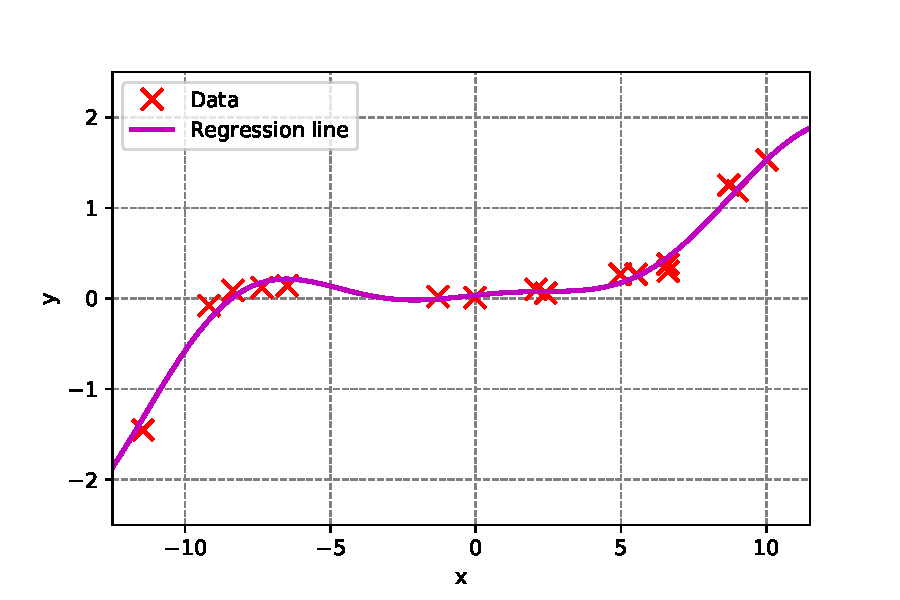
\includegraphics[scale=0.475]{18_advanced_regression/02_img/kernel_regression}}{Result of kernel ridge regression}{fig:kernel-regression}
\end{dwHeaderFrame}


% Section: Gaussian Process Regression
%______________________________________________________________________
\dwSection{Gaussian Process Regression}

% Introduction
\begin{dwHeaderFrame}{Introduction}
	\begin{itemize}
		\item Similarly to kernel ridge regression, Gaussian processes do not make any assumptions about the type of regression function (e.\,g. linear, quadratic, ...)
		\item It is non-parametric and a form of supervised learning:
		\begin{equation}
			h(\bm{x}) = \mathfrak{GP}(m(\bm{x}), \mathcal{K}(\bm{x}, \bm{x}'))
			\label{eq:gp}
		\end{equation}
		\item In \cref{eq:gp}, $m(\bm{x})$ denotes the mean function, whereas $\mathcal{K}(\bm{x}, \bm{x}')$ denotes the kernel function, which -- in the context of Gaussian processes -- is
			referred to as the covariance function.
		\item Definition of a Gaussian process:
		\begin{quote}
			Formally, a Gaussian process is a collection of random variables, any finite number of which has a \textbf{joint Gaussian distribution}.
		\end{quote}
	\end{itemize}
\end{dwHeaderFrame}


\begin{frame}
	\begin{itemize}
		\item Instead of modeling a distribution over parameters (cf. Bayesian regression), we model a \textbf{distribution over possible regression functions}.
		\item Thus, Gaussian processes extend multivariate Gaussian distributions to \textbf{infinite dimensions}.
		\begin{itemize}
			\item E.\,g. a function $f : \mathbb{R} \mapsto \mathbb{R}$ can be thought of as a sample from some infinite Gaussian distribution.
			\item Pick the function which maximizes the posterior distribution over functions.
		\end{itemize}
		\item The mean of the prior $m(\bm{x})$ distribution is usually set to 0 everywhere.
		\item In practice, the squared exponential function ($\widehat{=}$ RBF-kernel) is frequently used:
		\begin{equation}
			\mathcal{K}(\bm{x}, \bm{x}') = \sigma_f^2 \cdot \exp\left\{ \frac{-\Vert \bm{x} - \bm{x}' \Vert^2}{2 \cdot l^2} \right\}
		\end{equation}
		\item Hyper-Parameters:
		\begin{itemize}
			\item $\sigma_f^2$ denotes the maximum allowable covariance. It should be high for functions covering a broad range of the $y$-axis. If $\bm{x} \approx \bm{x}'$,
				$\mathcal{K}(\bm{x}, \bm{x}')$ approaches this maximum.
			\item $l$ (landmark) controls how much the data points influence each other.
		\end{itemize}
	\end{itemize}
\end{frame}


% Learning a Gaussian Process Model
\begin{dwHeaderFrame}{Learning a Gaussian Process Model}
	\begin{itemize}
		\item We are given a training data set $\mathcal{D}$ comprising $n$ observations:
		\begin{equation*}
			\mathcal{D} = \{ (\bm{x}^{(1)}, y^{(1)}), (\bm{x}^{(2)}, y^{(2)}), \dots, (\bm{x}^{(n)}, y^{(n)}) \} = \{ (\bm{x}^{(i)}, y^{(i)}) \}_{i=1}^n
		\end{equation*}
		\item Also, we have a query data point $\bm{x}_q$, for which $y_q$ has to be predicted.
		\item To do so, we compute the covariance between all example pairs.
		\item This results in three matrices $\bm{K}$ (matrix), $\bm{K}_*$ (vector) and $\bm{K}_{**}$ (scalar).
	\end{itemize}
\end{dwHeaderFrame}


\begin{frame}
	The matrices have the following form:

	\begin{align}
		\bm{K} &=
		\begin{bmatrix}
			\mathcal{K}(\bm{x}^{(1)}, \bm{x}^{(1)}) 	& \mathcal{K}(\bm{x}^{(2)}, \bm{x}^{(1)}) & \hdots & \mathcal{K}(\bm{x}^{(n)}, \bm{x}^{(1)}) 	\\
			\mathcal{K}(\bm{x}^{(1)}, \bm{x}^{(2)}) 	& \mathcal{K}(\bm{x}^{(2)}, \bm{x}^{(2)}) & \hdots & \mathcal{K}(\bm{x}^{(n)}, \bm{x}^{(2)}) 	\\
			\vdots 							& \vdots 							& \ddots & \vdots 							\\
			\mathcal{K}(\bm{x}^{(1)}, \bm{x}^{(n)}) 	& \mathcal{K}(\bm{x}^{(2)}, \bm{x}^{(n)}) & \hdots & \mathcal{K}(\bm{x}^{(n)}, \bm{x}^{(n)})
		\end{bmatrix} \\[8mm]
		\bm{K}_* &=
		\begin{bmatrix}
			\mathcal{K}(\bm{x}_q, \bm{x}^{(1)}) & \mathcal{K}(\bm{x}_q, \bm{x}^{(2)}) & \dots & \mathcal{K}(\bm{x}_q, \bm{x}^{(n)})
		\end{bmatrix}^{\intercal} \\[8mm]
		\bm{K}_{**} &= \mathcal{K}(\bm{x}_q, \bm{x}_q)
	\end{align}

	\dwAlertBox{$\bm{K}$ is a matrix (contains the similarities of training data pairs), $\bm{K}_*$ is a vector (contains similarities of the query data point with the training data),
		while $\bm{K}_{**}$ is actually a scalar (comparison of data point $\bm{x}_q$ to itself)!}
\end{frame}


\begin{frame}
	\begin{itemize}
		\item Since we assume that the data can be modeled as a sample from a multivariate Gaussian distribution, we can model the Gaussian process prior as follows:
		\begin{equation}
			\begin{bmatrix} \bm{y} \\ y_q \end{bmatrix} \thicksim
				\mathcal{N} \left(
					\bm{0}, 
					\begin{bmatrix} \bm{K} & \bm{K_*^{\intercal}} \\ \bm{K_*} & \bm{K_{**}} \end{bmatrix}
				\right)
		\end{equation}
		\item What we actually want is the \textbf{posterior distribution} $p(y_q \vert \bm{y})$: \textit{`Given the data, what is $y_q$?'}
		\item For Gaussian distributions, the posterior distribution can be computed analytically:
		\begin{equation}
			y_q \vert \bm{y} \thicksim \mathcal{N}(
				\underbracket{\bm{K}_* \bm{K}^{-1} \bm{y}}_{
					\substack{\text{\textbf{Matrix of}} \\ \text{\textbf{regr. coeff.}}}
				},
				\underbracket{\bm{K}_{**} - \bm{K}_* \bm{K}^{-1} \bm{K}_*^{\intercal}}_{
					\text{\textbf{Schur complement}}
				}
			)
		\end{equation}
		\item The mean of the posterior distribution is given by the \textbf{matrix of regression coefficients},
			its variance can be computed using the \textbf{Schur complement}.
		\item We can compute confidence intervals (e.\,g. 90\,\% | 95\,\% | 99\,\%):
		\begin{equation}
			(1.65\ |\ 1.96\ |\ 2.58) \cdot \sqrt{var(y_q)}
		\end{equation}
	\end{itemize}
\end{frame}


% Example
\begin{dwHeaderFrame}{Example}
	\dwFigure{
		\divideTwo{0.49}{
			\begin{figure}
	\centering
	\begin{tikzpicture}
    
  	  \begin{axis}[
			scale=0.4,
			xlabel={$x$},
			ylabel={$y$}
		]

			\pgfplotstableread{18_advanced_regression/05_data/datapoints_gp.txt} \datatable
			\addplot[only marks,mark=*,mark size=2,draw=black,fill=lightgray] table[x=x,y=y] from \datatable;

		\end{axis}
		
	\end{tikzpicture}
\end{figure}
		}{0.49}{
			\vspace*{3mm}
			\begin{figure}
	\centering
	\begin{tikzpicture}
    
  	  \begin{axis}[
			scale=0.4,
			xlabel={$x$},
			ylabel={$y$}
		]

			\pgfplotstableread{18_advanced_regression/05_data/datapoints_gp.txt} \datatable
			\addplot[only marks,mark=*,mark size=2,draw=black,fill=lightgray] table[x=x,y=y] from \datatable;

		\end{axis}
		
	\end{tikzpicture}
\end{figure}
		}
	}{Example data set for a Gaussian process}{fig:example-gp}
	
	\begin{itemize}
		\item Suppose $\sigma_f = 1.27, l = 1.00$. What is $y_q$ for $\bm{x}_q = 8$?
		\item Let's plot the prior distribution first.
	\end{itemize}
\end{dwHeaderFrame}


\begin{frame}
	\dwHeader{Prior distribution}
	\dwFigure{\begin{figure}
	\centering
	\begin{tikzpicture}
    
	  	 \begin{axis}[
			scale=0.6,
			minor tick num=5,
			grid=both,
	    			grid style={line width=.1pt, draw=gray!10},
	    			major grid style={line width=.2pt,draw=gray!50},
			x=40,
			y=16.5,
			xmin=-2.00,
			xmax=12.00,
			hide axis
		]
	
			\pgfplotstableread{18_advanced_regression/05_data/datapoints_gp.txt} \datatable
			\pgfplotstableread{18_advanced_regression/05_data/datapoints_gp_prior.txt} \datatablePrior
	
			% plot same random samples from distribution
			\addplot[dashed] table[x=x,y=sample1] from \datatablePrior;
			\addplot[dashed] table[x=x,y=sample2] from \datatablePrior;
			\addplot[dashed] table[x=x,y=sample3] from \datatablePrior;
			\addplot[dashed] table[x=x,y=sample4] from \datatablePrior;
			\addplot[dashed] table[x=x,y=sample5] from \datatablePrior;
	
			% plot mean and data points
			\addplot[draw=black,ultra thick] table[x=x,y=mu] from \datatablePrior;
			\addplot[only marks,mark=*,mark size=2.5,draw=black,fill=orange] table[x=x,y=y] from \datatable;

		\end{axis}
		
	\end{tikzpicture}
\end{figure}}{Prior distribution for the Gaussian process}{fig:gp-prior}
	\begin{itemize}
		\item Naturally, the prior does not fit the data well (we have not fitted the model yet).
		\item We have zero mean everywhere.
	\end{itemize}
\end{frame}


\begin{frame}
	\dwHeader{Posterior distribution}
	\dwFigure{\begin{figure}
	\centering
	\begin{tikzpicture}
    
	  	  \begin{axis}[
			scale=0.6,
			minor tick num=5,
			grid=both,
	    			grid style={line width=.1pt, draw=gray!10},
	    			major grid style={line width=.2pt,draw=gray!50},
			x=35,
			y=16.5,
			xmin=-3.51,
			xmax=13.51,
			hide axis
		]

			\pgfplotstableread{18_advanced_regression/05_data/datapoints_gp.txt} \datatable
			\pgfplotstableread{18_advanced_regression/05_data/datapoints_mu_sigma_gp.txt} \datatableMuSigma

			% plot confidence intervals
			\addplot[draw=none,name path=muPlusNineNine] table[x=x,y=muPlus99] from \datatableMuSigma;
			\addplot[draw=none,name path=muMinusNineNine] table[x=x,y=muMinus99] from \datatableMuSigma;
			\addplot[lightgray!30] fill between[of=muPlusNineNine and muMinusNineNine];
			\addplot[draw=none,name path=muPlusNineFive] table[x=x,y=muPlus95] from \datatableMuSigma;
			\addplot[draw=none,name path=muMinusNineFive] table[x=x,y=muMinus95] from \datatableMuSigma;
			\addplot[lightgray!60] fill between[of=muPlusNineFive and muMinusNineFive];
			\addplot[draw=none,name path=muPlusNineZero] table[x=x,y=muPlus90] from \datatableMuSigma;
			\addplot[draw=none,name path=muMinusNineZero] table[x=x,y=muMinus90] from \datatableMuSigma;
			\addplot[lightgray!80] fill between[of=muPlusNineZero and muMinusNineZero];

			% plot same random samples from distribution
			\addplot[dashed] table[x=x,y=sample1] from \datatableMuSigma;
			\addplot[dashed] table[x=x,y=sample2] from \datatableMuSigma;
			\addplot[dashed] table[x=x,y=sample3] from \datatableMuSigma;

			% plot mean and data points
			\addplot[draw=black,ultra thick] table[x=x,y=mu] from \datatableMuSigma;
			\addplot[only marks,mark=*,mark size=2.5,draw=black,fill=orange] table[x=x,y=y] from \datatable;

		\end{axis}

	\end{tikzpicture}
\end{figure}}{Posterior distribution for the Gaussian process}{fig:gp-posterior}
	\dwAlertBox{Wait a minute: Isn't this model overfitting the training data?}
\end{frame}


\begin{frame}
	\begin{itemize}
		\item The model clearly overfits the data as can be seen from the previous slide (the regression line goes through each training data point perfectly).
		\item This is because the model assumes the data to be \textbf{noise-free}.
		\item It is possible to add a little bit of noise, in order to deal with this easily ($\sigma_n$ is the variance of the noise):
		\begin{equation}
			\bm{K}_{\sigma_n} \longleftarrow \bm{K} + \sigma_n \bm{I}
		\end{equation}
		\item The updated formulas look like this:
		\begin{itemize}
			\item Matrix of regression coefficients (\textbf{same result as in kernel ridge regression}):
			\begin{equation}
				\bm{K_*} \bm{K}_{\sigma_n}^{-1} \bm{y}
			\end{equation} 
			\item Schur complement:
			\begin{equation}
				\bm{K}_{**} - \bm{K}_* \bm{K}_{\sigma_n}^{-1} \bm{K}_*^{\intercal}
			\end{equation}
		\end{itemize}
	\end{itemize}
\end{frame}


\begin{frame}
	\dwHeader{Prior distribution (with noise)}
	\dwFigure{\begin{figure}
	\centering
	\begin{tikzpicture}
    
	  	  \begin{axis}[
			scale=0.6,
			minor tick num=5,
			grid=both,
	    			grid style={line width=.1pt, draw=gray!10},
	    			major grid style={line width=.2pt,draw=gray!50},
			x=35,
			y=18,
			xmin=-3.51,
			xmax=13.51,
			hide axis
		]

			\pgfplotstableread{18_advanced_regression/05_data/datapoints_gp.txt} \datatable
			\pgfplotstableread{18_advanced_regression/05_data/datapoints_mu_sigma_gp_with_noise.txt} \datatableMuSigma

			% plot confidence intervals
			\addplot[draw=none,name path=muPlusNineNine] table[x=x,y=muPlus99] from \datatableMuSigma;
			\addplot[draw=none,name path=muMinusNineNine] table[x=x,y=muMinus99] from \datatableMuSigma;
			\addplot[lightgray!30] fill between[of=muPlusNineNine and muMinusNineNine];
			\addplot[draw=none,name path=muPlusNineFive] table[x=x,y=muPlus95] from \datatableMuSigma;
			\addplot[draw=none,name path=muMinusNineFive] table[x=x,y=muMinus95] from \datatableMuSigma;
			\addplot[lightgray!60] fill between[of=muPlusNineFive and muMinusNineFive];
			\addplot[draw=none,name path=muPlusNineZero] table[x=x,y=muPlus90] from \datatableMuSigma;
			\addplot[draw=none,name path=muMinusNineZero] table[x=x,y=muMinus90] from \datatableMuSigma;
			\addplot[lightgray!80] fill between[of=muPlusNineZero and muMinusNineZero];

			% plot same random samples from distribution
			\addplot[dashed] table[x=x,y=sample1] from \datatableMuSigma;
			\addplot[dashed] table[x=x,y=sample2] from \datatableMuSigma;
			\addplot[dashed] table[x=x,y=sample3] from \datatableMuSigma;

			% plot mean and data points
			\addplot[draw=black,ultra thick] table[x=x,y=mu] from \datatableMuSigma;
			\addplot[only marks,mark=*,mark size=2.5,draw=black,fill=orange] table[x=x,y=y] from \datatable;
			
		\end{axis}

	\end{tikzpicture}
\end{figure}}{Posterior distribution for the Gaussian process with noise}{fig:gp-posterior-noise}
\end{frame}


% Learning the Hyper-Parameters
\begin{dwHeaderFrame}{Learning the Hyper-Parameters}
	\begin{itemize}
		\item The results of Gaussian process regression depend heavily on the parameters $\{ \sigma_f, l \}$, which is why these parameters should be optimized for the task at hand.
		\item This can be down by maximizing the \textbf{marginal likelihood} (e.\,g. by using gradient ascent).
	\end{itemize}
	
	\dwInfoBox{The exact procedure is very involved and out of scope for this lecture.}
\end{dwHeaderFrame}


% Section: Support Vector Regression
%______________________________________________________________________
\dwSection{Support Vector Regression}

% Introduction
\begin{dwHeaderFrame}{Introduction}
	\begin{itemize}
		\item Support vector machines can be extended to regression problems, while preserving the property of sparseness.
		\item In ordinary least squares, we minimize a regularized error function given by:
		\begin{equation}
			\mathcal{J}(\bm{\theta}) = \frac{1}{2} \sum_{i=1}^n (\widehat{h}(\bm{x}^{(i)}) - y^{(i)})^2 + \frac{\lambda}{2} \Vert \bm{w} \Vert^2
		\end{equation}
		\item In the following, $\bm{\theta} = \{ \bm{w}, b \}$ and $\widehat{h}(\bm{x}) = \bm{w}^{\intercal} \varphi(\bm{x}) + b$.
		\item To obtain sparse solutions, the quadratic error is replaced by an \textbf{$\bm{\varepsilon}$-insensitive error function}, which gives zero error if the absolute difference between the
			prediction and the target is less than $\varepsilon$:
		\begin{equation}
			\ell_{\varepsilon}(\widehat{h}(\bm{x}) - y) =
			\begin{cases}
				0 									& \text{if $\vert \widehat{h}(\bm{x}) - y \vert < \varepsilon$} \\
				\vert \widehat{h}(\bm{x}) - y \vert - \varepsilon 	& \text{otherwise}
			\end{cases}
		\end{equation}
	\end{itemize}
\end{dwHeaderFrame}


\begin{frame}
	\dwFigure{\begin{figure}
	\centering
	\begin{tikzpicture}
    
		\draw[very thick,-stealth] (-5,0) -- (5,0) node[right] {$z$};
		\draw[very thick,-stealth] (0,0) -- (0,3) node[above] {$\ell(z)$};

		\draw[red,very thick] (-4,3) -- (-1,0) -- (1,0) -- (4,3);
		\draw[domain=-1.75:1.75,smooth,variable=\x,blue,very thick] plot ({\x},{\x*\x});

		\node at (-1,-0.5) {$-\varepsilon$};
		\node at (1,-0.5) {$\varepsilon$};
		\node at (0,-0.5) {0};
		
	\end{tikzpicture}
\end{figure}}
		{An $\varepsilon$-insensitive error function (red) compared to the quadratic error function (blue)}{fig:eps-insensitive-error}
\end{frame}


\begin{frame}
	\begin{itemize}
		\item We therefore minimize a regularized error function given by:
		\begin{equation}
			\mathcal{J}(\bm{\theta}) = C \sum_{i=1}^n \ell_{\varepsilon}(\widehat{h}(\bm{x}^{(i)}) - y^{(i)}) + \frac{1}{2} \Vert \bm{w} \Vert^2
		\end{equation}
		\item Analogously to support vector machines for classification, $C$ denotes the (inverse) regularization parameter.
		\item Again, we introduce slack variables:
		\begin{itemize}
			\item We now need two slack variables $\xi_i \ge 0$ and $\widehat{\xi}_i \ge 0$ for each data point $\bm{x}^{(i)}$.
			\item $\xi_i > 0$ corresponds to a point for which $y^{(i)} > \widehat{h}(\bm{x}^{(i)}) + \varepsilon$.
			\item $\widehat{\xi}_i \ge 0$ corresponds to a point for which $y^{(i)} < h(\bm{x}^{(i)}) - \varepsilon$.
		\end{itemize}
		\item The error function for support vector regression can then be rewritten as:
		\begin{equation}
			\mathcal{J}(\bm{\theta}) = C \sum_{i=1}^n (\xi_i + \widehat{\xi}_i) + \frac{1}{2} \Vert \bm{w} \Vert^2
			\label{eq:svr-error-function}
		\end{equation}
	\end{itemize}
\end{frame}


\begin{frame}
	\divideTwo{0.29}{
		Illustration of SVM regression, showing the regression curve together with the $\varepsilon$-insensitive `tube'. Also shown are examples
		of the slack variables $\xi$ and $\widehat{\xi}$. \\[3mm]

		Points above the $\varepsilon$-tube have $\xi > 0$ and $\widehat{\xi} = 0$, points below the tube have $\xi = 0$ and $\widehat{\xi} > 0$.
		Points inside the tube are characterized by $\xi = \widehat{\xi} = 0$.
	}{0.69}{
		\vspace*{3mm}
		\dwFigure{\begin{figure}
	\centering
	\begin{tikzpicture}
    
		\draw[very thick,-stealth] (0,0) -- (7,0) node[right] {$x$};
		\draw[very thick,-stealth] (0,0) -- (0,5) node[above] {$\widehat{h}(x)$};

		\fill[red!30] (1,0.5) -- ++(0,1) --  plot[domain=1:6,smooth,variable=\x] ({\x},{0.00416667*\x^5-0.0625*\x^4+0.395833*\x^3-1.4375*\x^2+3.35*\x-0.75})
			-- ++(0,-1) -- plot[domain=6:1,smooth,variable=\x] ({\x},{0.00416667*\x^5-0.0625*\x^4+0.395833*\x^3-1.4375*\x^2+3.35*\x-1.75}) -- cycle;

		\draw[domain=1:6,smooth,variable=\x,red,very thick] plot ({\x},{0.00416667*\x^5-0.0625*\x^4+0.395833*\x^3-1.4375*\x^2+3.35*\x-1.25});

		\node[anchor=west] at (6.25,4) {$\widehat{h}(x)$};
		\node[anchor=west] at (6.25,4.75) {$\widehat{h}(x) + \varepsilon$};
		\node[anchor=west] at (6.25,3.25) {$\widehat{h}(x) - \varepsilon$};

		\node at (3.75,3.75) {$\xi > 0$};
		\node at (3.25,1.5) {$\widehat{\xi}_i > 0$};
		
	\end{tikzpicture}
\end{figure}}{Illustration of support vector regression}{fig:svr}
	}
\end{frame}


% Optimization
\begin{dwHeaderFrame}{Optimization}
	\begin{itemize}
		\item The cost function given by \cref{eq:svr-error-function} must be minimized subject to the constraints:
		\begin{align}
			\xi_i 			&\ge 0 							\\
			\widehat{\xi}_i 	&\ge 0 							\\
			y^{(i)} 		&\le h(\bm{x}^{(i)}) + \varepsilon + \xi_i 	\\
			y^{(i)} 		&\ge h(\bm{x}^{(i)}) - \varepsilon - \widehat{\xi}_i
		\end{align}
		\item This can be achieved by introducing Lagrange multipliers $\alpha_i \ge 0, \widehat{\alpha}_i \ge 0, \mu_i \ge 0$ and $\widehat{\mu}_i \ge 0$:
		\begin{align}
			\nonumber
			\mathcal{L}
				&= C \sum_{i=1}^n (\xi_i + \widehat{\xi}_i) + \frac{1}{2} \Vert \bm{w} \Vert^2 - \sum_{i=1}^n (\mu_i \xi_i + \widehat{\mu}_i \widehat{\xi}_i) \\
				&\phantom{=} - \sum_{i=1}^n \alpha_i (\varepsilon + \xi_i + \widehat{h}(\bm{x}^{(i)}) - y^{(i)}) -
					\sum_{i=1}^n \widehat{\alpha}_i (\varepsilon + \widehat{\xi}_i - \widehat{h}(\bm{x}^{(i)}) + y^{(i)})
		\end{align}
	\end{itemize}
\end{dwHeaderFrame}


\begin{frame}
	\dwHeader{Derivatives of $\mathcal{L}$}
	\begin{alignat}{2}
		\frac{\partial\mathcal{L}}{\partial \bm{w}} 		&\overset{!}{=} 0 \qquad &&\Rightarrow \qquad \bm{w} = \sum_{i=1}^n (\alpha_i - \widehat{\alpha}_i) \varphi(\bm{x}^{(i)})
		\label{eq:derivative-w}																													\\[3mm]
		\frac{\partial\mathcal{L}}{\partial b} 			&\overset{!}{=} 0 \qquad &&\Rightarrow \qquad \sum_{i=1}^n (\alpha_i - \widehat{\alpha}_i) = 0 						\\[3mm]
		\frac{\partial\mathcal{L}}{\partial \xi_i} 			&\overset{!}{=} 0 \qquad &&\Rightarrow \qquad \alpha_i + \mu_i = C
		\label{eq:derivative-xi}																													\\[3mm]
		\frac{\partial\mathcal{L}}{\partial \widehat{\xi}_i} 	&\overset{!}{=} 0 \qquad &&\Rightarrow \qquad \widehat{\alpha}_i + \widehat{\mu}_i = C
		\label{eq:derivative-xi-hat}
	\end{alignat}

	\dwInfoBox{We can use these results to obtain the dual formulation which has to be maximized.}
\end{frame}


\begin{frame}
	\dwHeader{Dual formulation}
	\begin{itemize}
		\item The dual formulation is given by:
		\begin{equation}
			\mathcal{L}(\bm{\alpha}, \bm{\widehat{\alpha}}) = -\frac{1}{2} \sum_{i=1}^n \sum_{j=1}^n (\alpha_i - \widehat{\alpha}_i) (\alpha_j - \widehat{\alpha}_j)
				\mathcal{K}(\bm{x}^{(i)}, \bm{x}^{(j)}) - \varepsilon \sum_{i=1}^n (\alpha_i + \widehat{\alpha}_i) + \sum_{i=1}^n (\alpha_i - \widehat{\alpha}_i) y^{(i)}
		\end{equation}
		\item The dual is expressed in terms of a kernel function $\mathcal{K}(\bm{x}, \bm{x}')$.
		\item Maximize the dual function: $\max_{\bm{\alpha}, \bm{\widehat{\alpha}}} \mathcal{L}(\bm{\alpha}, \bm{\widehat{\alpha}})$
		\item Again, this is a constraint optimization problem which is optimized subject to:
		\begin{alignat}{2}
			0 	&\le \alpha_i 			&&\le C \\
			0 	&\le \widehat{\alpha}_i 	&&\le C
		\end{alignat}
		\item We again have the \textbf{box constraints} which directly follow from the fact that the Lagrange multipliers have to be $\ge 0$
			together with \cref{eq:derivative-xi} and \cref{eq:derivative-xi-hat}.
	\end{itemize}
\end{frame}


\begin{frame}
	\begin{itemize}
		\item Substituting \cref{eq:derivative-w} into $\widehat{h}(\bm{x})$, we see that predictions for new inputs can be made using:
		\begin{equation}
			\widehat{h}(\bm{x}) = \sum_{i=1}^n (\alpha_i - \widehat{\alpha}_i) \mathcal{K}(\bm{x}, \bm{x}^{(i)}) + b
			\label{eq:svr-prediction}
		\end{equation}
		\item The support vectors are those data points for which $\alpha_i \ne 0$ or $\widehat{\alpha}_i \ne 0$. Such points either lie on the boundary of the
			$\varepsilon$-tube or outside the tube. All points within the tube have $\alpha_i = \widehat{\alpha}_i = 0$.
		\item It is again a \textbf{sparse solution}, since we only need the support vectors for the prediction.
	\end{itemize}
\end{frame}


% Karush-Kuhn-Tucker Conditions
\begin{dwHeaderFrame}{Karush-Kuhn-Tucker Conditions}
	\begin{itemize}
		\item The \textbf{Karush-Kuhn-Tucker (KKT) conditions} state that at the solution, the product of dual variables and constraints must vanish.
		\item The KKT conditions for support vector regression are given by:
		\begin{align}
			\alpha_i (\varepsilon + \xi_i + \widehat{h}(\bm{x}^{(i)}) - y^{(i)}) 					&= 0
			\label{eq:kkt-1}														\\[2mm]
			\widehat{\alpha}_i (\varepsilon + \widehat{\xi}_i - \widehat{h}(\bm{x}^{(i)}) + y^{(i)}) 	&= 0
			\label{eq:kkt-2}														\\[2mm]
			\overbracket{(C - \alpha_i)}^{\mu_i} \xi_i									&= 0
			\label{eq:kkt-3}														\\[2mm]
			\underbracket{(C - \widehat{\alpha}_i)}_{\widehat{\mu}_i} \widehat{\xi}_i 			&= 0
		\end{align}
	\end{itemize}
	
	\dwInfoBox{We can derive useful results from the KKT conditions (cf. next slide).}
\end{dwHeaderFrame}


\begin{frame}
	\begin{itemize}
		\item First of all, we note that $\alpha_i$ can only be \textbf{non-zero}, if $\varepsilon + \xi_i + \widehat{h}(\bm{x}^{(i)}) - y^{(i)} = 0$. This implies that the data point either lies
			on the upper boundary of the $\varepsilon$-tube ($\xi_i = 0$) or above it ($\xi_i > 0$).
		\item Analogous: $\widehat{\alpha}_i$
		\item The two constraints $\varepsilon + \xi_i + \widehat{h}(\bm{x}^{(i)}) - y^{(i)}$ and $\varepsilon + \widehat{\xi}_i - \widehat{h}(\bm{x}^{(i)}) + y^{(i)}$ are incompatible.
			This can be seen by adding them together and noting that $\xi_i, \widehat{\xi}_i$ are non-negative and $\varepsilon$ is strictly positive. So for every data point
			$\bm{x}^{(i)}$, either $\alpha_i$ or $\widehat{\alpha}_i$ (or both) must be zero.
		\item Parameter $b$ in \cref{eq:svr-prediction} can be found by considering a data point for which $0 < \alpha_i < C$ ($\widehat{=}$ support vector).
			From \cref{eq:kkt-3} it must have $\xi_i = 0$. Therefore, according to \cref{eq:kkt-1} it must satisfy $\varepsilon + \widehat{h}(\bm{x}^{(i)}) - y^{(i)} = 0$.
		\item For $b$ we obtain:
		\begin{align}
			b 
				&= y^{(i)} - \varepsilon - \bm{w}^{\intercal} \varphi(\bm{x}^{(i)}) \\[1mm]
				&= y^{(i)} - \varepsilon - \sum_{j=1}^n (\alpha_j - \widehat{\alpha}_j) \mathcal{K}(\bm{x}^{(i)}, \bm{x}^{(j)})
		\end{align}
		\item In practice, it is better to consider all support vectors to find $b$ (average).
	\end{itemize}
\end{frame}


% Example
\begin{dwHeaderFrame}{Example}
	\dwFigure{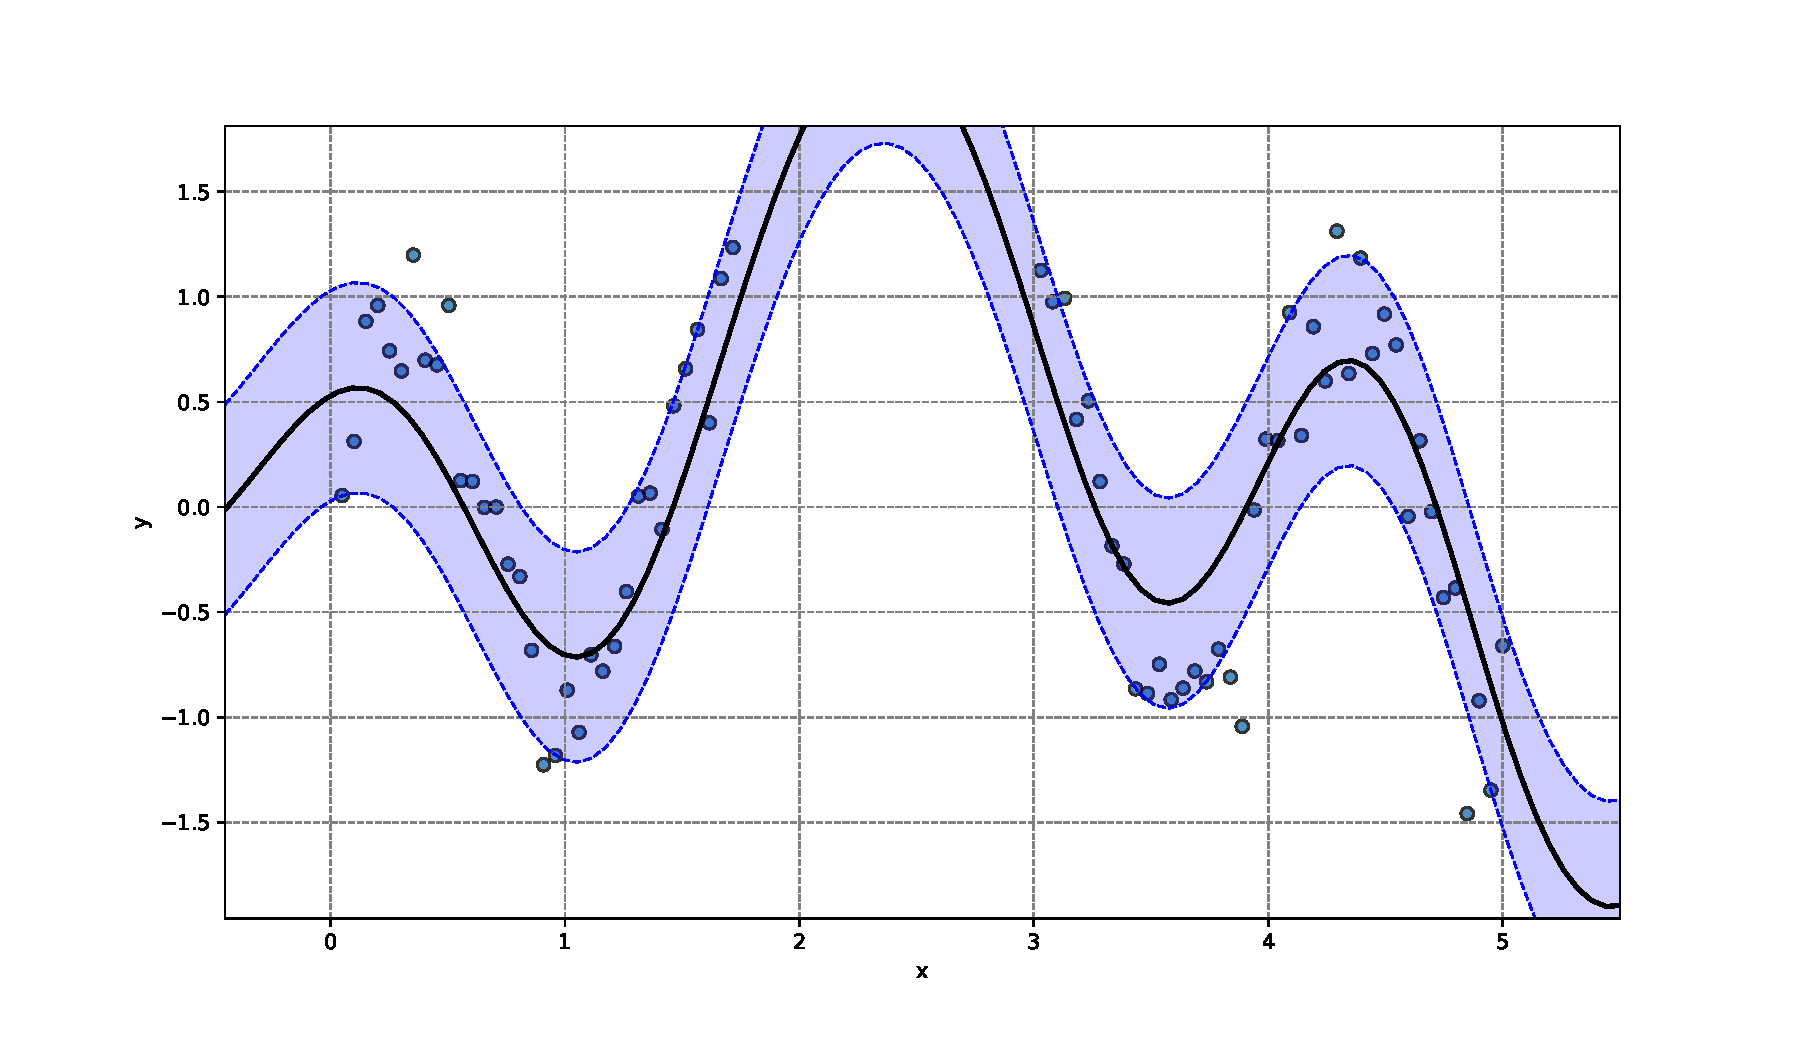
\includegraphics[scale=0.275]{18_advanced_regression/02_img/svr_example}}
		{Example of support vector regression using \texttt{scikit-learn}}{fig:svr-example}
\end{dwHeaderFrame}

\end{document}
